\def\mytitle{CIRCLE ASSIGNMENT}
\def\myauthor{PANJUGALA SHASHIKALA}
\def\contact{sashipanjugala@gmail.com}
\def\mymodule{Future Wireless Communication (FWC)}
\documentclass[10pt, a4paper]{article}
\usepackage[a4paper,outer=1.5cm,inner=1.5cm,top=1.75cm,bottom=1.5cm]{geometry}
\twocolumn
\usepackage{setspace}
\doublespacing
\usepackage{graphicx}
\graphicspath{{./images/}}
\usepackage[colorlinks,linkcolor={black},citecolor={blue!80!black},urlcolor={blue!80!black}]{hyperref}
\usepackage[parfill]{parskip}
\usepackage{lmodern}
\usepackage{tikz}
	\usepackage{physics}
%\documentclass[tikz, border=2mm]{standalone}
\usepackage{karnaugh-map}
%\documentclass{article}
\usepackage{tabularx}
\usepackage{circuitikz}
\usetikzlibrary{calc}
\usepackage{amsmath}
\usepackage{amssymb}
\renewcommand*\familydefault{\sfdefault}
\usepackage{watermark}
\usepackage{lipsum}
\usepackage{xcolor}
\usepackage{listings}
\usepackage{float}
\usepackage{titlesec}
\usepackage{amsmath}
\providecommand{\mtx}[1]{\mathbf{#1}}
\titlespacing{\subsection}{1pt}{\parskip}{3pt}
\titlespacing{\subsubsection}{0pt}{\parskip}{-\parskip}
\titlespacing{\paragraph}{0pt}{\parskip}{\parskip}
\newcommand{\figuremacro}[5]{
    \begin{figure}[#1]
        \centering
        \includegraphics[width=#5\columnwidth]{#2}
        \caption[#3]{\textbf{#3}#4}
        \label{fig:#2}
    \end{figure}
}
\newcommand{\myvec}[1]{\ensuremath{\begin{pmatrix}#1\end{pmatrix}}}
\let\vec\mathbf
\lstset{
frame=single, 
breaklines=true,
columns=fullflexible
}

\thiswatermark{\centering \put(-15,-100.0){\includegraphics[scale=0.4]{iith.png}} }
\title{\mytitle}
\author{\myauthor\hspace{1em}\\\contact\\FWC22097 -\hspace{0.5em}IITH\hspace{0.5em}\mymodule\hspace{6em}}
\date{}


\begin{document}
\maketitle


\section{Question}
\textbf{\textit{Q(6), C , Section-A, Chapter-8:}A variable circle passes through the fixed point A(p,q) and touches the x-axis. The locus of the other end of the diameter through  A is }

\section{Solution}
\raggedright 

\begin{figure}[h!]
\centering
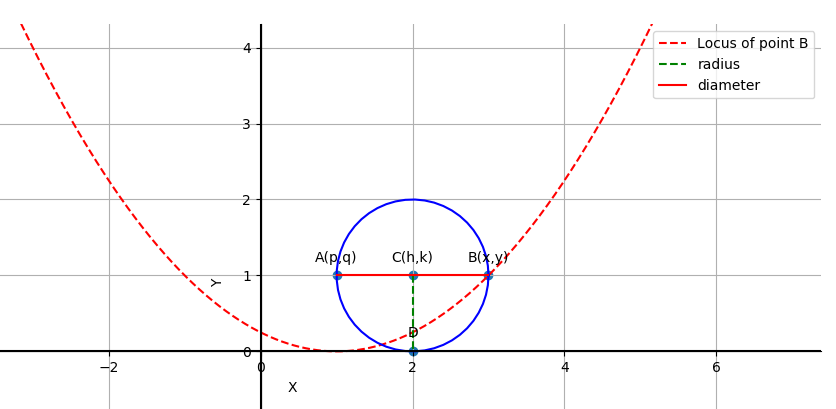
\includegraphics[scale=0.3]{circle1.png} \\
\end{figure}

\vspace{0.25cm}
Given the circle passes through the point $$\vec{A}=\myvec{ p \\ q }$$\\
Let the other end of the diameter through A be $$\vec{B}=\myvec{ x \\ y }$$ and the centre be $\vec{C}$. \\
By using section formula, we can find the centre C as\\
\begin{equation}
\vec{C}=\frac{1}{2}(\vec{A}+\vec{B})
\end{equation}
$$\vec{C}=\frac{1}{2}\myvec{p+x \\ q+y}$$ 
We know that AB is the diameter of the circle.And from figure we can find the radius as $r=\frac{q+y}{2}$. \\ We can write\\
\begin{equation}
||\vec{B-A}||= 2r
\end{equation}
Squaring on both sides, we get
\begin{equation}
||\vec{B-A}||^2= 4r^2
\end{equation}
\begin{equation}
||\vec{B-A}||^2=||\vec{A}||^2+||\vec{B}||^2-2{\vec{B}}^{\top}\vec{A}
\end{equation}
substituting equation (4), in equation (3)
\begin{equation}
||\vec{A}||^2+||\vec{B}||^2-2{\vec{B}}^{\top}\vec{A}=4r^2
\end{equation}
By solving the above equation we get,
\begin{equation}
\vec{A}^{\top}\vec{A}+\vec{B}^{\top}\vec{B}-2{\vec{B}}^{\top}\vec{A}=4r^2
\end{equation}
\begin{equation}
\vec{A}^{\top}\vec{A}+\vec{B}^{\top}\vec{B}-2{\vec{B}}^{\top}\vec{A}-4r^2=0
\end{equation}

Equation (7) is the required equation,which is the equation of parabola
\boldmath

$\vec{x}^{\top}\vec{V}\vec{x}+2\vec{u}^{\top}\vec{x}+f=0$
\unboldmath

where,
$$
\vec{V}=
\begin{bmatrix}
1 & 0 \\
0 & 0 \\
\end{bmatrix}
$$

$$\vec{u}=\myvec{ -1 \\ -2 }$$\\
$$f=p^2$$




\vspace{3cm}
Get the python code of the figures from
\begin{table}[h]
\large
\centering
\framebox{
\url{https://github.com/PanjugalaShashikala/FWC_2022097/tree/main/Circle/code/circle.py}}
\bibliographystyle{ieeetr}
\end{table}

\end{document}